%%%%%%%%%%%%%%%%%%%%%%%%%%%%%%%%%%%%%%%%%%%%%%%%%%%%%%%%%%%%%%%%%%%%%
%
% Complete documentation on the extended LaTeX markup used for Insight
% documentation is available in ``Documenting Insight'', that is part
% of the standard documentation for Insight.  It may be found online
% at:
%
%                    http://www.itk.org
%
%%%%%%%%%%%%%%%%%%%%%%%%%%%%%%%%%%%%%%%%%%%%%%%%%%%%%%%%%%%%%%%%%%%%%

\documentclass{InsightSoftwareGuide}

\usepackage[dvips]{graphicx}
\usepackage{times,lscape,url}

\usepackage[latin1]{inputenc}

\usepackage{tikz}

\usepackage{color}

\definecolor{listcomment}{rgb}{0.0,0.5,0.0}
\definecolor{listkeyword}{rgb}{0.0,0.0,0.5}
\definecolor{listnumbers}{gray}{0.65}
\definecolor{listlightgray}{gray}{0.955}
\definecolor{listwhite}{gray}{1.0}

\usepackage{listings}
\newcommand{\lstsetcpp}
{
\lstset{frame = tb,
       framerule = 0.25pt,
       float,
       fontadjust,
       backgroundcolor={\color{listlightgray}},
       basicstyle = {\ttfamily\footnotesize},
       keywordstyle = {\ttfamily\color{listkeyword}\textbf},
       identifierstyle = {\ttfamily},
       commentstyle = {\ttfamily\color{listcomment}\textit},
       stringstyle = {\ttfamily},
       showstringspaces = false,
       showtabs = false,
       numbers = none,
       numbersep = 6pt,
       numberstyle={\ttfamily\color{listnumbers}},
       tabsize = 2,
       language=[ANSI]C++,
       floatplacement=!h
       }
}
\newcommand{\lstsetpython}
{
\lstset{language=Python
        }
}
\newcommand{\lstsetjava}
{
\lstset{language=Java
        }
}


\newif\ifitkFullVersion
\itkFullVersiontrue
%\itkFullVersionfalse

\newif\ifitkPrintedVersion
\itkPrintedVersiontrue
%\itkPrintedVersionfalse


%%%%%%%%%%%%%%%%%%%%%%%%%%%%%%%%%%%%%%%%%%%%%%%%%%%%%%%%%%%%%%%%%%
%
%  hyperref should be the last package to be loaded.
%
%%%%%%%%%%%%%%%%%%%%%%%%%%%%%%%%%%%%%%%%%%%%%%%%%%%%%%%%%%%%%%%%%%
\ifitkPrintedVersion
\usepackage[dvips,
pdftitle={The Orfeo ToolBox CookBook, a guide for non-developpers},
pdfauthor={CNES},
pdfsubject={Remote Sensing, Orfeo, Pleiades, Cosmo Skymed},
pdfkeywords={image processing, Remote sensing, Guide},
pdfpagemode={UseOutlines},
bookmarks,bookmarksopen,
pdfstartview={FitH},
backref,
colorlinks,linkcolor={black},citecolor={black},urlcolor={black},
]{hyperref}
\else
\usepackage[dvips,
pdftitle={The Orfeo ToolBox CookBook, a guide for non-developpers},
pdfauthor={CNES},
pdfsubject={Remote Sensing, Orfeo, Pleiades, Cosmo Skymed},
pdfkeywords={image processing, Remote sensing, Guide},
pdfpagemode={UseOutlines},
bookmarks,bookmarksopen,
pdfstartview={FitH},
backref,
colorlinks,linkcolor={blue},citecolor={blue},urlcolor={blue},
]{hyperref}
\fi

\usepackage{amsmath,amssymb,amsfonts}
\usepackage{bbm}

\def\logoCNES{../Art/logoVectoriel.pdf}

\newtheorem{algo}{Algorithm}
\newtheorem{defin}{Definition}

\title{The Orfeo ToolBox CookBook, a guide for non-developpers\\ Updated
  for OTB-3.2}

\author{OTB Development Team}

\authoraddress{
  \url{http://www.orfeo-toolbox.org}\\
  e-mail: \email{otb@cnes.fr}
}

\date{\today}


% actually write the .idx file
\makeindex

\setcounter{tocdepth}{3}

%%%%%%%%%%%%%%%%%%%%%%%%%%%%%%%%%%%%%%%%%%%%%%%%%%%%%%%%%%%%%%%%%%%
%
%           Begin Document
%
%%%%%%%%%%%%%%%%%%%%%%%%%%%%%%%%%%%%%%%%%%%%%%%%%%%%%%%%%%%%%%%%%%%

\begin{document}

\ifitkPrintedVersion
\fi

\maketitle

\frontmatter

\hyperbaseurl{http://www.orfeo-toolbox.org}

\lstsetcpp

%%%%%%%%%%%%%%%%%%%%%%%%%%%%%%%%%%%%%%%%%%
%
%  Page with OTB logo
%
%%%%%%%%%%%%%%%%%%%%%%%%%%%%%%%%%%%%%%%%%%
\cleardoublepage

\begin{minipage}[t][10cm][b]{\textwidth}
\center
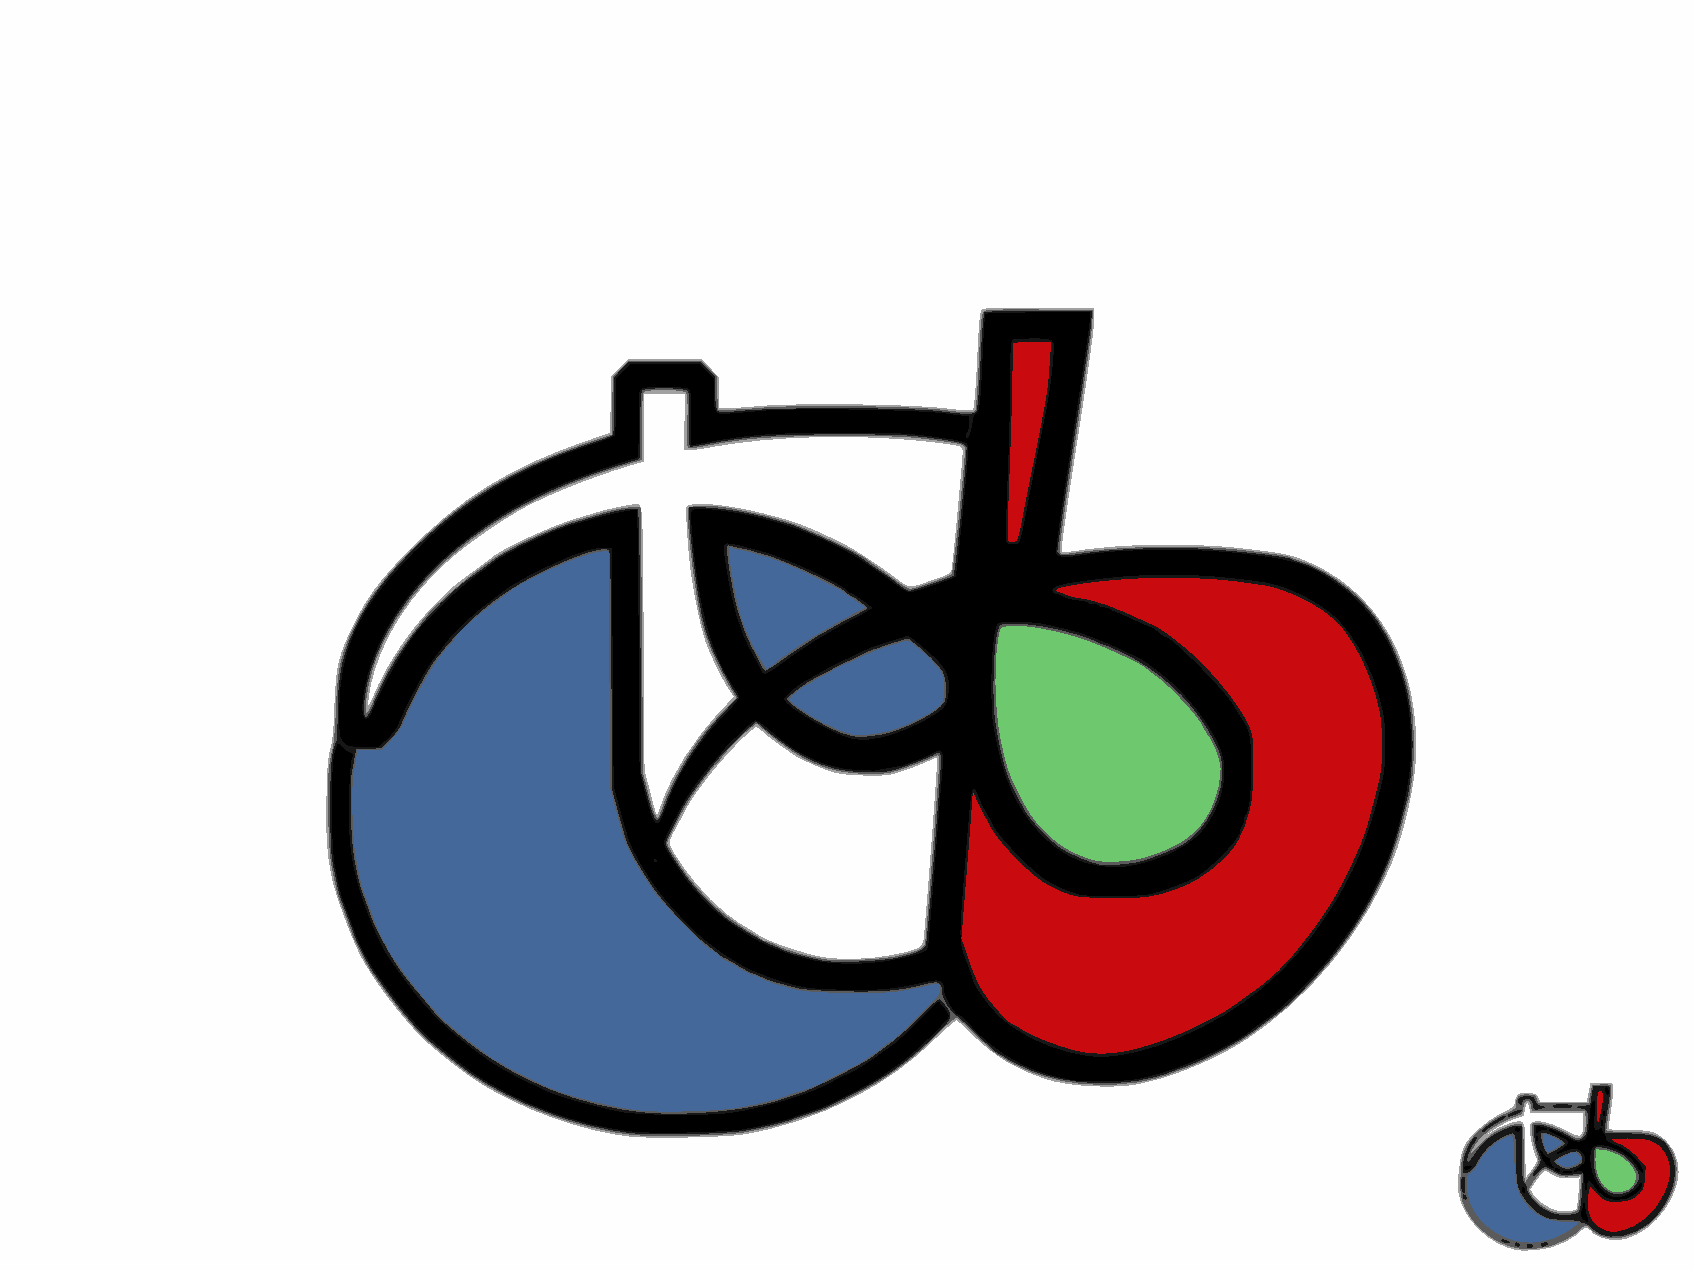
\includegraphics[width=0.5\textwidth]{../Art/logoVectoriel.pdf}
\large
\begin{center}
\emph{The ORFEO Toolbox is not a black box.}\\
\end{center}
\hspace{8cm} Ch.D.
\normalsize
\end{minipage}

%%%%%%%%%%%%%%%%%%%%%%%%%%%%%%%%%%%%%%%%%%%%%%
%
% remove headings from the following material
\pagestyle{plain}
%
%%%%%%%%%%%%%%%%%%%%%%%%%%%%%%%%%%%%%%%%%%%%%%

%%\ifitkPrintedVersion
%% % We want this material to fit on two pages
\small

\chapter*{About the Cover}

Creating the cover image demonstrating the capabilities of the toolkit was a
challenging task.\footnote{The source code for the cover is available from
InsightDocuments/SoftwareGuide/Cover/Source/.} Given that the origins of ITK
are with the Visible Human Project it seemed appropriate to create an image
utilizing the VHP data sets, and it was decided to use the more recently
acquired Visible Woman dataset.  Both the RGB cryosections and the CT scans
were combined in the same scene.

\begin{description}

\item [Removing the Gel.]
The body of the Visible Woman was immersed in a block of gel during the
freezing process. This gel appears as a blue material in the cryogenic data.
To remove the gel, the joint histogram of RGB values was computed. This
resulted in an 3D image of $256\times256\times256$ pixels. The histogram
image was visualized in VolView.\footnote{VolView is a commercial product
from Kitware. It supports ITK plug-ins and is available as a free viewer or
may be licensed with advanced functionality. See
http://www.kitware.com/products/volview.html for information.} The cluster
corresponding to the statistical distribution of blue values was identified
visually, and a separating plane was manually defined in RGB space. The
equation of this plane was subsequently used to discriminate pixels in the
gel from pixels in the anatomical structures. The gel pixels were zeroed out
and the RGB values on the body were preserved.

\item[The Skin.]
The skin was easy to segment once the gel was removed. A simple region
growing algorithm was used requiring seed points in the region previously
occupied by the gel and then set to zero values. An anti-aliasing filter was
applied in order to generate an image of pixel type float where the surface
was represented by the zero set. This data set was exported to VTK where a
contouring filter was used to extract the surface and introduce it in the VTK
visualization pipeline.

\item[The Brain.]
The visible part of the brain represents the surface of the gray matter.  The
brain was segmented using the vector version of the confidence connected
image filter.  This filter implements a region growing algorithm that starts
from a set of seed points and adds neighboring pixels subject to a condition
of homogeneity.

The set of sparse points obtained from the region growing algorithm was
passed through a mathematical morphology dilation in order to close holes and
then through a binary median filter. The binary median filter has the
outstanding characteristic of being very simple in implementation by applying
a sophisticated effect on the image. Qualitatively it is equivalent to a
curvature flow evolution of the iso-contours. In fact the binary median
filter as implemented in ITK is equivalent to the majority filter that
belongs to the family of voting filters classified as a subset of the
\emph{Larger than Life} cellular automata. Finally, the volume resulting from
the median filter was passed through the anti-aliasing image filter. As
before, VTK was used to extract the surface.

\item[The Neck Musculature.]
The neck musculature was not perfectly segmented. Indeed, the resulting
surface is a fusion of muscles, blood vessels and other anatomical
structures. The segmentation was performed by applying the
VectorConfidenceConnectedImageFilter to the cryogenic dataset. Approximately
60 seed points were manually selected and then passed to the filter as
input. The binary mask produced by the filter was dilated with a mathematical
morphology filter and smoothed with the BinaryMedianImageFilter. The
AntiAliasBinaryImageFilter was used at the end to reduce the pixelization
effects prior to the extraction of the iso-surface with vtkContourFilter.

\item[The Skull.]
The skull was segmented from the CT data set and registered to the cryogenic
data. The segmentation was performed by simple thresholding, which was good
enough for the cover image. As a result, most of the bone structures are
actually fused together. This includes the jaw bone and the cervical
vertebrae.

\item[The Eye.] 
The eye is charged with symbolism in this image. This is due in part because
the motivation for the toolkit is the analysis of the Visible Human data,
and in part because the name of the toolkit is \emph{Insight}.

The first step in processing the eye was to extract a sub-image of
$60\times60\times60$ pixels centered around the eyeball from the RGB
cryogenic data set. This small volume was then processed with the vector
gradient anisotropic diffusion filter in order to increase the homogeneity of
the pixels in the eyeball.

The smoothed volume was segmented using the
VectorConfidenceConnectedImageFilter using 10 seed points. The resulting
binary mask was dilated with a mathematical morphology filter with a
structuring element of radius one, then smoothed with a binary mean image
filter (equivalent to majority voting cellular automata). Finally the mask
was processed with the AntiAliasBinaryImageFilter in order to generate a
float image with the eyeball contour embedded as a zero set.

\item[Visualization.]
The visualization of the segmentation was done by passing all the binary
masks through the AntiAliasBinaryImageFilter, generating iso-contours with
VTK filters, and then setting up a VTK Tcl script. The skin surface was
clipped using the vtkClipPolyDataFilter using the implicit function
vtkCylinder. The vtkWindowToImageFilter proved to be quite useful for
generating the final high resolution rendering of the scene ($3000\times3000$
pixels).

\item[Cosmetic Postprocessing.]
We have to confess that we used Adobe Photoshop to post-process the image. In
particular, the background of the image was adjusted using Photoshop's color
selection. The overall composition of the image with the cover text and
graphics was also performed using Photoshop.

\end{description}

\normalsize

%%\fi

%\chapter*{Foreword}
\noindent


Beside the Pleiades (PHR) and Cosmo-Skymed (CSK) systems developments
forming ORFEO, the dual and bilateral system (France - Italy) for
Earth Observation, the ORFEO Accompaniment Program was set up, to
prepare, accompany and promote the use and the exploitation of the
images derived from these sensors.

The creation of a preparatory
program\footnote{http://smsc.cnes.fr/PLEIADES/A\_prog\_accomp.htm} is
needed because of:
\begin{itemize}
\item the new capabilities and performances of the ORFEO systems
  (optical and radar high resolution, access capability, data quality,
  possibility to acquire simultaneously in optic and radar),
\item the implied need of new methodological developments : new
  processing methods, or adaptation of existing methods,
\item the need to realise those new developments in very close
  cooperation with the final users for better integration of new
  products in their systems.

\end{itemize}

This program was initiated by CNES mid-2003 and will last until mid
2013.  It consists in two parts, between which it is necessary to keep
a strong interaction:
\begin{itemize}
\item A Thematic part,
\item A Methodological part.
\end{itemize}

The Thematic part covers a large range of applications (civil and
defence), and aims at specifying and validating value added products
and services required by end users. This part includes consideration
about products integration in the operational systems or processing
chains. It also includes a careful thought on intermediary structures
to be developed to help non-autonomous users. Lastly, this part aims
at raising future users awareness, through practical demonstrations
and validations.

The Methodological part objective is the definition and the
development of tools for the operational exploitation of the
submetric optic and radar images (tridimensional aspects, changes
detection, texture analysis, pattern matching, optic radar
complementarities). It is mainly based on R\&D studies and doctorate
and post-doctorate researches.

In this context, CNES\footnote{http://www.cnes.fr} decided to develop
the \emph{ORFEO ToolBox} (OTB), a set of algorithms encapsulated in a
software library. The goals of the OTB is to capitalise a methological
\textit{savoir faire} in order to adopt an incremental development
approach aiming to efficiently exploit the results obtained in the
frame of methodological R\&D studies.

All the developments are based on FLOSS (Free/Libre Open Source
Software) or existing CNES developments. OTB is distributed under the
C\'eCILL licence,
\url{http://www.cecill.info/licences/Licence_CeCILL_V2-en.html}.

OTB is implemented in C++ and is mainly based on
ITK\footnote{http://www.itk.org} (Insight Toolkit).


%% L'environnement de l'OTB est mis en place par l'outil CMake\footnote{http://www.cmake.org},
%% permettant ainsi de g\'{e}rer les proc\'{e}dures de compilation, g\'{e}n\'{e}ration et d'installation et ce quelque sois la plate forme cible.

%% Dans un souci d'homog\'{e}n\'{e}isation, l'OTB est con\c{c}ue et d\'{e}velopp\'{e}e suivant la philosophie et les principes \'{e}dict\'{e}s
%% par la biblioth\`{e}que ITK (programmation g\'{e}n\'{e}rique, m\'{e}canisme des \emph{Object Factories}, \emph{Smart pointers}, exceptions, \emph{Multi-Threading}, etc...).
%% Ces principes sont pr\'{e}sent\'{e}s dans le paragraphe \emph{3.2 Essential System Concepts} du guide ITK \url{http://www.itk.org/ItkSoftwareGuide.pdf}

%% Enfin, la m\'{e}thodologie de d\'{e}veloppement appliqu\'{e}e s'appuie sur une approche it\'{e}rative bas\'{e}e sur la programmation agile :
%% le sch\'{e}ma de d\'{e}veloppement suit le cycle \'{e}dict\'{e}e par la m\'{e}thodolgie de l'eXtreme Programming (XP)\footnote{http://www.xprogramming.com}.



%% Ce document constitue le guide d'utilisation et de d\'{e}veloppement de l'OTB. La version la plus r\'{e}cente de ce document est accessible \`{a}
%% \url{http://smsc.cnes.fr/PLEIADES/Fr/A_prog_accomp.htm/OTB/otbSoftwareGuide.pdf}.



\chapter*{Foreword}
\noindent

%%%%%%%%%%%%%%%%%%%%%%%%%%%%%%%%%%%%%%%%%%%%%%%%%%%%%%%%%
%
% Insert Table of Contents; List of Figures and Tables
%
%%%%%%%%%%%%%%%%%%%%%%%%%%%%%%%%%%%%%%%%%%%%%%%%%%%%%%%%%


%%%%%%%%%%%%%%%%%%%%%%%%%%%%%%%%%%%%%%%%%%%%%%
%
% enable headings from the following material
\pagestyle{normal}
%
%%%%%%%%%%%%%%%%%%%%%%%%%%%%%%%%%%%%%%%%%%%%%%
\small
\tableofcontents
\listoffigures
\listoftables
\normalsize

%%%%%%%%%%%%%%%%%%%%%%%%%%%%%%%%%%%%%%%%%
%
% Begin technical content
%
%%%%%%%%%%%%%%%%%%%%%%%%%%%%%%%%%%%%%%%%%

\mainmatter

\chapter{Introduction}

\chapter{Installation}

\chapter{OTB-Applications}

\chapter{Monteverdi}

\chapter{Recipes}

\section{Optical radiometric calibration}

\end{document}



